The results will proceed by an analysis of the metrics discussed previously. 

\subsection{Cumulative Rewards \& Cumulative Failures during Training}

    \begin{minipage}{.5\textwidth}
      \centering
        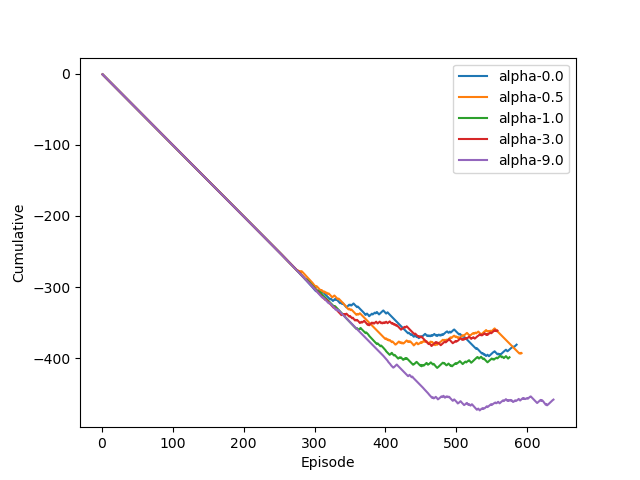
\includegraphics[width=1.1\linewidth]{figures/cumulative-minimal.png}
        \captionof{figure}{Cumulative rewards @ minimal}
        \label{fig:cumulativeminimal}
    \end{minipage} %
    \begin{minipage}{.5\textwidth}
        \centering
        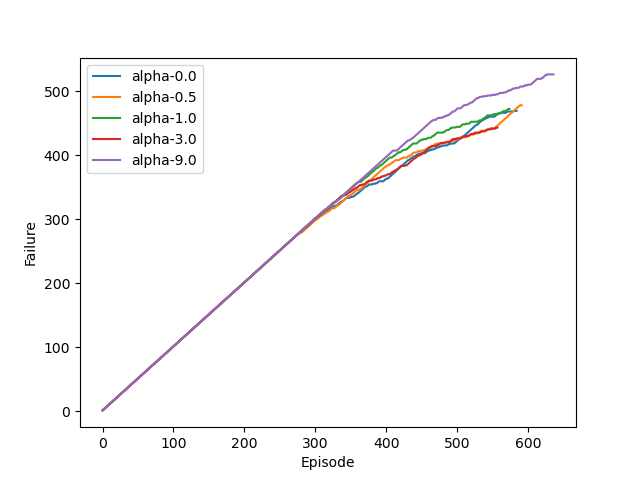
\includegraphics[width=1.1\linewidth]{figures/failures-minimal.png}
        \captionof{figure}{Cumulative failures @ minimal}
        \label{fig:failuresminimal}
    \end{minipage}


    \begin{minipage}{.5\textwidth}
        \centering
          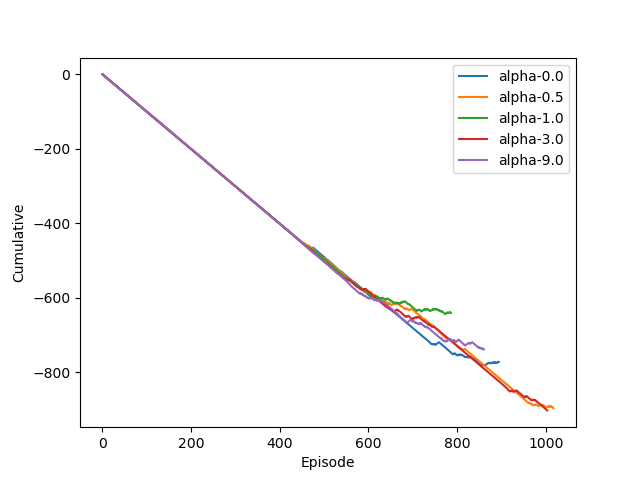
\includegraphics[width=1.1\linewidth]{figures/cumulative-intermediate.png}
          \captionof{figure}{Cumulative rewards @ intermediate}
          \label{fig:cumulativeminimal}
      \end{minipage} %
      \begin{minipage}{.5\textwidth}
          \centering
          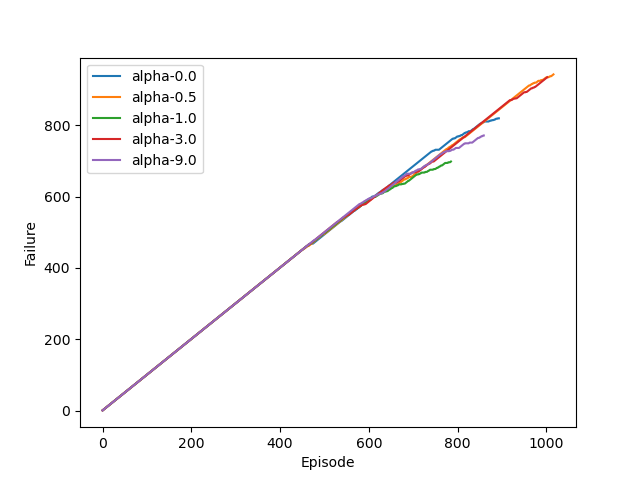
\includegraphics[width=1.1\linewidth]{figures/failures-intermediate.png}
          \captionof{figure}{Cumulative failures @ intermediate}
          \label{fig:failuresminimal}
      \end{minipage} %
      
    \smallskip
  We see an overall similar pattern over our different configurations of obstacles, 
  all alphas start at a similar pace before diverging as to when the agent learns not to crash. 
  The cumulative rewards mostly stabilizes in the minimal setting, where alpha 0.5 is the first to reach a plateau. 
  In the intermediate setting, some alphas reach a plateau much earlier than RL by itself. 
  Precisely, in the intermediate case, alpha 1 is the first to reach a plateau, while alpha 3 and alpha 9 fail to ever reach one. 
  Note that the number of episodes are different for each setting because all have been trained over 250k frames, so the less episodes ran, 
  the quicker the agent learnt to not crash and thus can exhaust its
  frames `living' rather than accumulate episodes of failures. 
  In both the minimal setting, the one that has the least number of episodes is 3.0 while in the intermediate case, that is alpha 1.0.

\subsection{Failures during Training}

  \begin{figure}[H]
    \centering
    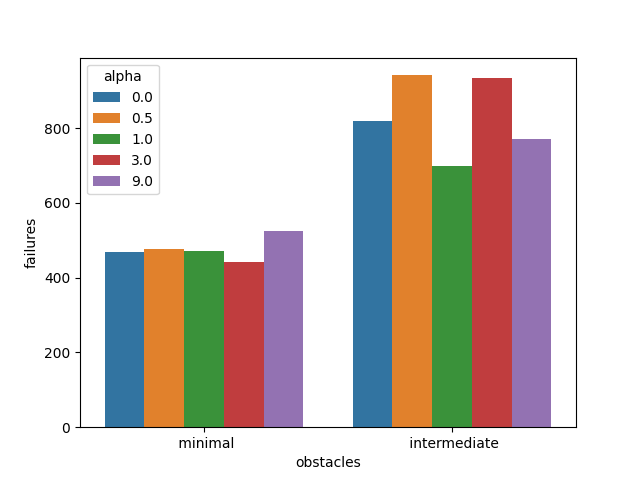
\includegraphics[scale=0.8]{figures/sfe.png}
    \caption{Overall failures during Training}
    \label{fig:sfe}
  \end{figure}

  Although, there is no substantial changes in the overall failures when dealing with minimal obstacles, as the scenario gets more complex, i.e. intermediate number of obstacles in the world, 
  we see that alpha 1 allows the agent to crash less before learning. 
  %
  During training, some alphas allows us to ensure more safety to the agent, as in minimize its crashes. As the agent fails less, it is able to increase its cumulative rewards earlier. 
  We are left with the question of evaluating performance during deployement to see if this added safety takes away from the learned policy, either in terms of average frames to reach the target, or 
  more failures during deployement. We also see that different alphas behave very differently with no apparent evidence as to which is optimal. 

  \subsection{Policy during Deployement}

        \begin{minipage}{.5\textwidth}
            \centering
            \begin{tabular}{||c c c||} 
                \hline
                Alphas & Frames & Reward \\ [0.5ex] 
                \hline\hline
                0.0 & 962 $\pm$ 173 & 0.80 $\pm$ 0.42 \\ 
                \hline
                0.5 & 1000 $\pm$ 11 & 0.90 $\pm$ 0.00 \\
                \hline
                1.0 & 764 $\pm$ 332 & 0.1 $\pm$ 0.96 \\
                \hline
                3.0 & 983 $\pm$ 110 & 0.82 $\pm$ 0.38 \\
                \hline
                9.0 & 967 $\pm$ 143 & 0.76 $\pm$ 0.50 \\ [1ex] 
                \hline
               \end{tabular}
               \captionof{table}{Mean frames and rewards @ minimal}
          \end{minipage} %
          \begin{minipage}{.5\textwidth}
              \centering
              \begin{tabular}{||c c c||} 
                \hline
                Alphas & Frames & Reward \\ [0.5ex] 
                \hline\hline
                0.0 & 872 $\pm$ 248 & 0.41 $\pm$ 0.84 \\ 
                \hline
                0.5 & 652 $\pm$ 366 & -0.29 $\pm$ 0.95 \\
                \hline
                1.0 & 872 $\pm$ 284 & 0.39 $\pm$ 0.84 \\
                \hline
                3.0 & 998.9 $\pm$ 74 & 0.84 $\pm$ 0.33 \\
                \hline
                9.0 & 474 $\pm$ 368 & -0.59 $\pm$ 0.81 \\ [1ex] 
                \hline
               \end{tabular}
               \captionof{table}{Mean frames and rewards @ intermediate}
          \end{minipage}

          In the minimal setting, 0.5 has the least variance and the highest mean reward per episode. All alphas have positive mean rewards, meaning they succeed more than fail, 
          although 1.0 has the most variance and is the least performing. For all other alphas, their performance is comparable to RL by itself, 0.5 is the only one that outperforms. 
          In the intermediate setting, 0.5 and 9.0 are the worst performing, averaging a negative reward per episode. RL by itself performs similarly to 1.0 and is outperformed by 3.0 that averages the highest mean reward, 
          and has the most average of steps, meaning it lives the longest. 

  \subsection{Failures during Deployement}


\begin{figure}[H]
    \centering
    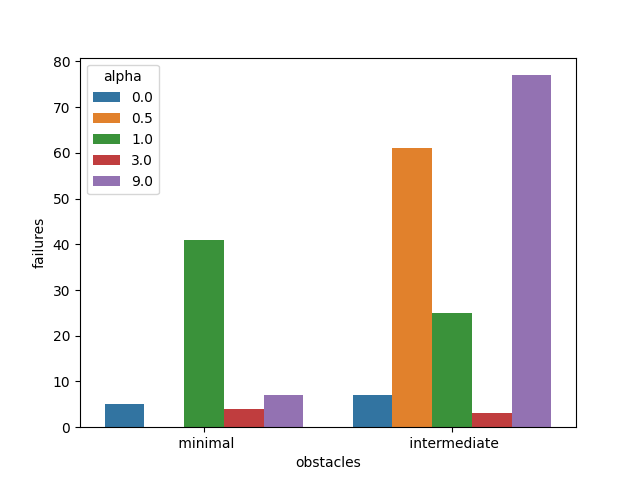
\includegraphics[scale=0.8]{figures/sfe-deployement.png}
    \caption{Overall failures during Deployement}
    \label{fig:sfe}
  \end{figure}

  We see that during deployement, the most unsafe policy is 9.0 for the intermediate setting, and 1.0 for the minimal setting, which agrees with our discussion over the deployed policies above. 
  Although in the minimal setting, during training, 9.0 crashes more than all other alphas, it still behaves better than 1.0.
  On the other hand, 0.5 performs the best across all other alphas in the minimal setting. It is the least uncertain during deployement, and does not crash.
  During training in the minimal setting, 0.5 was also the first to reach a plateau, meaning it had the most opportunity to learn to minimize crashing. 
  In the intermediate setting, no other alpha is more safe than RL by itself, except 3.0 by a small margin, which also outperforms it in the learned policy when it comes to averaged rewards.


  \section{Discussion}
  Our above results show us that there is no apparent difference over
  alphas during deployement, except that some result in `worse' safety outcomes, i.e. crashing more than RL by itself.  
  However, during training, several alphas, allow us to minimize failures, and thus might allow us to train agents in the real world where safety is important. 
  For `good' alphas, there does not seem to be a loss in optimality of policy, rather some allow the agent to behave better than RL by itself, especially given the average reward per episode. 
  To confirm those results, it would be interesting to extrapolate the alphas for more obstacles, where learning has to be done faster OR increase the number of frames to train, to allow all alphas 
  to reach a plateau and thus compare optimality in terms of average frames, i.e. how quickly does the agent reach the goal. 






